\subsection{Введение}
В данной части лабораторной работы произведены измерения действующих значений входного напряжения, тока и фазового сдвига между ними для девяти различных двухполюсников, а также произведены сравнения результатов с расчётными значениями.

\subsection{Параметры элементов исследуемых схем}
\begin{enumerate}
	\item Расчёт амплитуды синусоидального напряжения:
	      \[
		      U_m =  U_{\text{д}} \cdot \sqrt{2} = 6 \cdot \sqrt{2} = 8.485 \, \text{В}
	      \]

	\item Известные значения:
	      \[
		      \begin{gathered}
			      U_{\text{д}} = 6 \, \text{В}, \psi_{\text{н}} = 0^{\circ}, f = 19.894 \, \text{Гц}, R_1 = 30 \, \text{Ом}, R_k = 5 \, \text{Ом} \\
			      L_k = 23.094 \, \text{мГн}, C = 71.454 \, \text{мкФ}
		      \end{gathered}
	      \]

\end{enumerate}

\subsection{Общие расчёты}
\begin{enumerate}
	\item Угловая частота:
	      \[
		      \omega = 2 \pi f = 2 \cdot 3.1416 \cdot 19.894 \approx 125 \, \text{рад/с} \\
	      \]

	\item Реактивная составляющая сопротивления ёмкостного элемента:
	      \[
		      X_c = \frac{1}{\omega C} = \frac{1}{125 \cdot 71.454 \cdot 10^{-6}} = 111.96 \, \text{Ом}
	      \]

	\item Реактивная составляющая сопротивления индуктивного элемента:
	      \[
		      X_L = \omega L = 125 \cdot 23.094 \cdot 10^{-3} = 2.887 \, \text{Ом}
	      \]

	\item Реактивная проводимость ёмкостного элемента:
	      \[
		      B_c = \omega C = 125 \cdot 71.454 \cdot 10^{-6} = 0.00893 \, \text{См}
	      \]

	\item Реактивная проводимость индуктивного элемента:
	      \[
		      B_k = \frac{X_L}{R_k^2 + X_L^2} = \frac{2.887}{5^2 + (2.887)^2} = 0.0866 \, \text{См}
	      \]
\end{enumerate}


\subsection{Двухполюсник 1}
\subsubsection{Схема исследуемой цепи}
\begin{figure}[H]
	\centering
	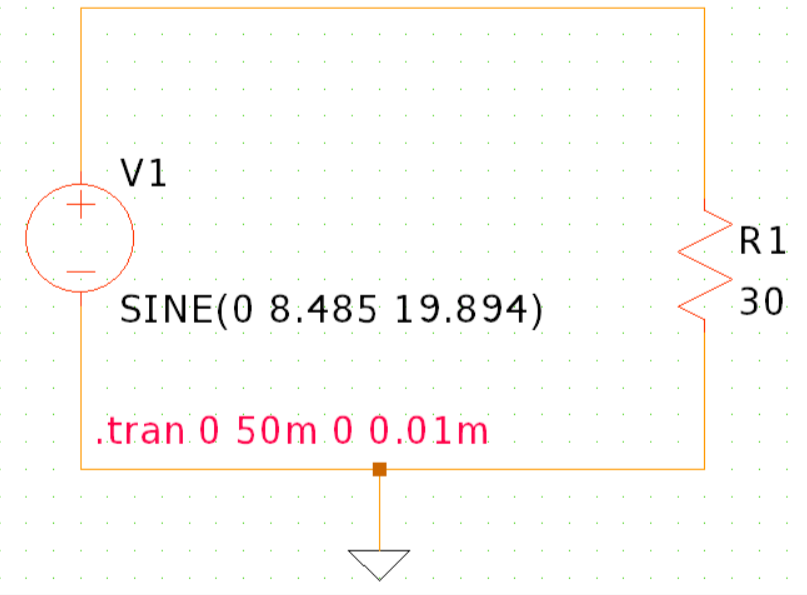
\includegraphics[width=1\textwidth]{./data/schema1}
	\caption{Схема замещения Двухполюсника 1 в LTspice.}
\end{figure}
\subsubsection{Расчётные формулы и расчёты}
\begin{enumerate}
	\item Расчёт действующего тока в цепи:
	      \[
		      \begin{gathered}
			      I = \frac{U}{Z} = \frac{U}{\sqrt{R^2 + X^2}} \\
			      X = 0, R = R_1 \implies I = \frac{U}{R_1} = \frac{6}{30} = 0.2 \, \text{А}
		      \end{gathered}
	      \]
	\item Расчёт фазового сдвига:
	      \[
		      \phi = \arctan\left(\frac{0}{R_1}\right) = 0^{\circ}
	      \]
\end{enumerate}

\subsubsection{Вектора входного напряжения и тока}
\begin{figure}[H]
	\centering
	\begin{tikzpicture}[scale=2.0]

		% Draw the grid
		\draw[very thin, gray] (-1.2,-1.2) grid (2.2,2.2);

		% Draw the axes
		\draw[->] (-1.2,0) -- (2.2,0) node[right] {$+1$};
		\draw[->] (0,-1.2) -- (0,2.2) node[above] {$+j$};

		% Draw the first vector (red) for current (I)
		\draw[->, red, thick] (0,0) -- (0.249,0) node[end, below] {$I = 0.249 \, \text{А}$};

		% Draw the second vector (blue) for voltage (U)
		\draw[->, blue, thick] (0,0) -- (0.6,0);
		\node[above right, blue] at (0.6, 0) {$U = 6 \, \text{В}$};

		% Draw the angle label
		\draw (0.1,0) arc[start angle=0, end angle=0, radius=1cm];
		\node[above right] at (-0.03,0) {\scriptsize $\phi = 0^{\circ}$};

	\end{tikzpicture}
\end{figure}


\subsection{Двухполюсник 2}
\subsubsection{Схема исследуемой цепи}
\begin{figure}[H]
	\centering
	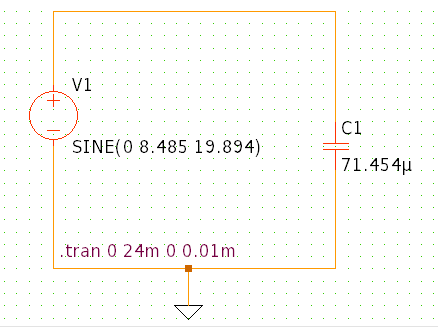
\includegraphics[width=0.8\textwidth]{./data/schema2}
	\caption{Схема замещения Двухполюсника 2 в LTspice.}
\end{figure}
\subsubsection{Расчётные формулы и расчёты}
\begin{enumerate}
	\item Расчёт действующего тока в цепи:
	      \[
		      \begin{gathered}
			      I = \frac{U}{Z} = \frac{U}{\sqrt{R^2 + X^2}} \\
			      X = -X_C, R = 0 \implies I = \frac{U}{X_C} = \frac{6}{111.96} = 0.0536 \, \text{А}
		      \end{gathered}
	      \]
	\item Расчёт фазового сдвига:
	      \[
		      \phi = \arctan\left(-\inf\right) = -90^{\circ}
	      \]
\end{enumerate}

\subsubsection{Вектора входного напряжения и тока}
\begin{figure}[H]
	\centering
	\begin{tikzpicture}[scale=1.8]

		% Draw the grid
		\draw[very thin, gray] (-1.2,-1.2) grid (2.2,2.2);

		% Draw the axes
		\draw[->] (-1.2,0) -- (2.2,0) node[right] {$+1$};
		\draw[->] (0,-1.2) -- (0,2.2) node[above] {$+j$};

		% Draw the current vector (red) for current (I) with a phase shift of -90 degrees
		\draw[->, red, thick] (0,0) -- (0,0.536) node[end, right] {$I = 0.0536 \, \text{А}$};

		% Draw the voltage vector (blue) for voltage (U)
		\draw[->, blue, thick] (0,0) -- (0.6,0) node[end, below] {$U = 6 \, \text{В}$};

		% Draw the phase angle arc (from U to I)
		\draw[thick] (0.2,0) arc[start angle=0, end angle=90, radius=0.2];
		\node at (0.55,0.2) {\scriptsize $\phi = -90^\circ$};

		\node[below left] at (0,0) {$0$};

	\end{tikzpicture}
\end{figure}


\subsection{Двухполюсник 3}
\subsubsection{Схема исследуемой цепи}
\begin{figure}[H]
	\centering
	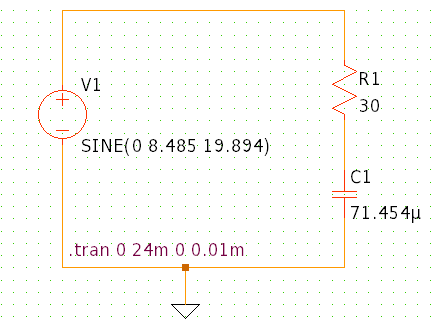
\includegraphics[width=0.5\textwidth]{./data/schema3}
	\caption{Схема замещения Двухполюсника 3 в LTspice.}
\end{figure}
\subsubsection{Расчётные формулы и расчёты}
\begin{enumerate}
	\item Расчёт действующего тока в цепи:
	      \[
		      \begin{gathered}
			      I = \frac{U}{Z} = \frac{U}{\sqrt{R^2 + X^2}} \\
			      X = -X_C, R = R_1 \implies I = \frac{U}{\sqrt{R_1^2+X_C^2}} = \frac{6}{\sqrt{30^2+111.96^2}} = 0.0518 \, \text{А}
		      \end{gathered}
	      \]
	\item Расчёт фазового сдвига:
	      \[
		      \phi = \arctan\left(\frac{-X_C}{R_1}\right) = \arctan\left(\frac{-111.96}{30}\right) = -75^{\circ}
	      \]
\end{enumerate}

\subsubsection{Вектора входного напряжения и тока}
\[
	\begin{gathered}
		I_x = I \cos(\phi), I_y = I sin(\phi) \\
		I_x = 0.0518 \cdot \cos(75^\circ) = 0.0134 \, \text{А}, \quad
		I_y = 0.0518 \cdot \sin(75^\circ) = 0.05 \, \text{А}
	\end{gathered}
\]
\begin{figure}[H]
	\centering
	\begin{tikzpicture}[scale=4.0]

		% Draw the grid
		\draw[very thin, gray] (-1.2,-1.2) grid (2.2,2.2);

		% Draw the axes
		\draw[->] (-1.2,0) -- (2.2,0) node[right] {$+1$};
		\draw[->] (0,-1.2) -- (0,2.2) node[above] {$+j$};

		% Draw the current vector (red) with a phase shift of -75 degrees
		\draw[->, red, thick] (0,0) -- ({0.518*cos(75)}, {0.518*sin(75)})
		node[end, right] {$I = 0.0518 \, \text{А}$};
		\draw[gray, thin, dashed] ({0.518*cos(75)},0) node[start, below, red] {\scriptsize0.0134} -- ({0.518*cos(75)}, {0.518*sin(75)});
		\draw[gray, thin, dashed] (0,{0.518*sin(75)}) node[start, left, red] {\scriptsize0.05} -- ({0.518*cos(75)}, {0.518*sin(75)});


		% Draw the voltage vector (blue) for voltage (U)
		\draw[->, blue, thick] (0,0) -- (1.8,0) node[end, above] {$U = 6 \, \text{В}$};

		% Draw the phase angle arc (from U to I)
		\draw[thick] (0.18,0) arc[start angle=0, end angle=75, radius=0.18];
		\node at (0.36,0.18) {\small $\phi = -75^\circ$};

		% Labels for the axis
		\node[below left] at (0,0) {$0$};

	\end{tikzpicture}
\end{figure}


\subsection{Двухполюсник 4}
\subsubsection{Схема исследуемой цепи}
\begin{figure}[H]
	\centering
	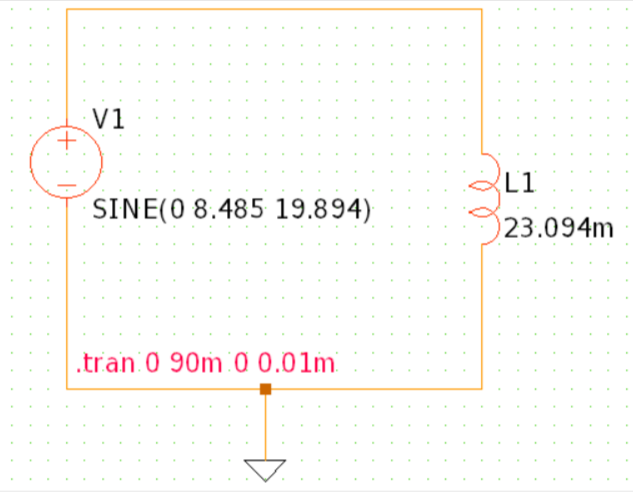
\includegraphics[width=1\textwidth]{./data/schema4}
	\caption{Схема замещения Двухполюсника 4 в LTspice.}
\end{figure}
\subsubsection{Расчётные формулы и расчёты}
\begin{enumerate}
	\item Расчёт действующего тока в цепи:
	      \[
		      \begin{gathered}
			      I = \frac{U}{Z} = \frac{U}{\sqrt{R^2 + X^2}} \\
			      X = X_L, R = R_k \implies I = \frac{U}{\sqrt{R_k^2+X_L^2}} = \frac{6}{\sqrt{5^2+2.887^2}} = 1.039 \, \text{А}
		      \end{gathered}
	      \]
	\item Расчёт фазового сдвига:
	      \[
		      \phi = \arctan\left(\frac{X_L}{R_k}\right) = \arctan\left(\frac{2.887}{5}\right) = 30.7^{\circ}
	      \]
\end{enumerate}

\subsubsection{Вектора входного напряжения и тока}
\[
	\begin{gathered}
		I_x = I \cos(\phi), I_y = I sin(\phi) \\
		I_x = 1.039 \cdot \cos(-30.7^\circ) = 0.893 \, \text{А}, \quad
		I_y = 1.039 \cdot \sin(-30.7^\circ) = -0.531 \, \text{А}
	\end{gathered}
\]
\begin{figure}[H]
	\centering
	\begin{tikzpicture}[scale=5.0]

		% Draw the grid
		\draw[very thin, gray] (-1.2,-1.2) grid (2.2,2.2);

		% Draw the axes
		\draw[->] (-1.2,0) -- (2.2,0) node[right] {$+1$};
		\draw[->] (0,-1.2) -- (0,2.2) node[above] {$+j$};

		% Draw the current vector (red) with a phase shift of -75 degrees
		\draw[->, red, thick] (0,0) -- ({1.039*cos(-30.7)}, {1.039*sin(-30.7)})
		node[end, right] {$I = 1.039 \, \text{А}$};
		\draw[gray, thin, dashed] ({1.039*cos(-30.7)},0) node[start, below, red] {\scriptsize0.893} -- ({1.039*cos(-30.7)}, {1.039*sin(-30.7)});
		\draw[gray, thin, dashed] (0,{1.039*sin(-30.7)}) node[start, left, red] {\scriptsize0.531} -- ({1.039*cos(-30.7)}, {1.039*sin(-30.7)});


		% Draw the voltage vector (blue) for voltage (U)
		\draw[->, blue, thick] (0,0) -- (0.6,0) node[end, above] {$U = 6 \, \text{В}$};

		% Draw the phase angle arc (from U to I)
		\draw[thick] (0.18,0) arc[start angle=0, end angle=-30.7, radius=0.18];
		\node at (0.4,-0.07) {\scriptsize $\phi = 30.7^\circ$};

		% Labels for the axis
		\node[below left] at (0,0) {$0$};

	\end{tikzpicture}
\end{figure}


\subsection{Двухполюсник 5}
\subsubsection{Схема исследуемой цепи}
\begin{figure}[H]
	\centering
	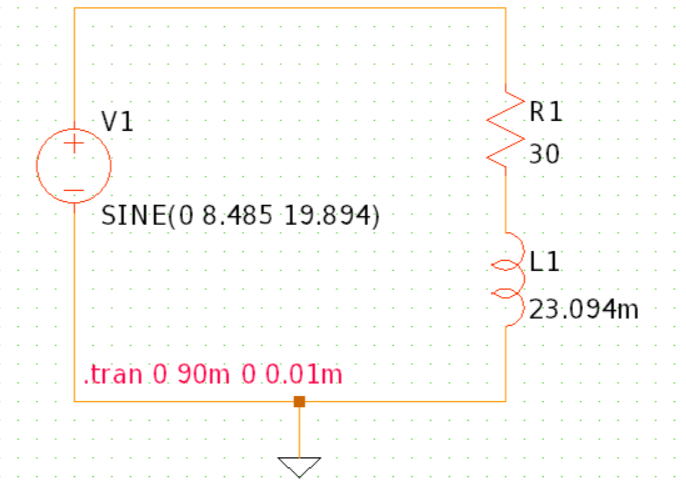
\includegraphics[width=1\textwidth]{./data/schema5}
	\caption{Схема замещения Двухполюсника 5 в LTspice.}
\end{figure}
\subsubsection{Расчётные формулы и расчёты}
\begin{enumerate}
	\item Расчёт действующего тока в цепи:
	      \[
		      \begin{gathered}
			      I = \frac{U}{Z} = \frac{U}{\sqrt{R^2 + X^2}} \\
			      X = X_L, R = R_1 + R_k \implies I = \frac{U}{\sqrt{(R_1+R_k)^2+X_L^2}} = \frac{6}{\sqrt{(30+5)^2+2.887^2}} \\
			      \\
			      = 0.171 \, \text{А}
		      \end{gathered}
	      \]
	\item Расчёт фазового сдвига:
	      \[
		      \phi = \arctan\left(\frac{X_L}{R_1+R_k}\right) = \arctan\left(\frac{2.887}{30+5}\right) = 4.72^{\circ}
	      \]
\end{enumerate}

\subsubsection{Вектора входного напряжения и тока}
\[
	\begin{gathered}
		I_x = I \cos(\phi), I_y = I sin(\phi) \\
		I_x = 0.171 \cdot \cos(-4.72^\circ) = 0.17 \, \text{А}, \quad
		I_y = 0.171 \cdot \sin(-4.72^\circ) = -0.014 \, \text{А}
	\end{gathered}
\]
\begin{figure}[H]
	\centering
	\begin{tikzpicture}[scale=25.0]

		% Draw the grid
		\draw[very thin, gray] (-0.05,-0.3) grid (0.65,0.5);

		% Draw the axes
		\draw[->] (-0.05,0) -- (0.65,0) node[right] {$+1$};
		\draw[->] (0,-0.4) -- (0,0.5) node[above] {$+j$};

		% Draw the current vector (red) with a phase shift of -75 degrees
		\draw[->, red, thick] (0,0) -- ({0.171*cos(-4.72)}, {0.171*sin(-4.72)})
		node[end, right] {$I = 0.171 \, \text{А}$};
		\draw[gray, thin, dashed] ({0.171*cos(-4.72)},0) node[start, above, red] {\scriptsize0.17} -- ({0.171*cos(-4.72)}, {0.171*sin(-4.72)});
		\draw[gray, thin, dashed] (0,{0.171*sin(-4.72)}) node[start, left, red] {\scriptsize-0.014} -- ({0.171*cos(-4.72)}, {0.171*sin(-4.72)});


		% Draw the voltage vector (blue) for voltage (U)
		\draw[->, blue, thick] (0,0) -- (0.6,0) node[end, above] {$U = 6 \, \text{В}$};

		% Draw the phase angle arc (from U to I)
		\draw[thick] (0.11,0) arc[start angle=0, end angle=-4.72, radius=0.11];
		\node at (0.145,-0.006) {\scriptsize $\phi = 4.7^\circ$};

		% Labels for the axis
		\node[below left] at (0.005,0.005) {\scriptsize$0$};

	\end{tikzpicture}
\end{figure}


\subsection{Двухполюсник 6}
\subsubsection{Схема исследуемой цепи}
\begin{figure}[H]
	\centering
	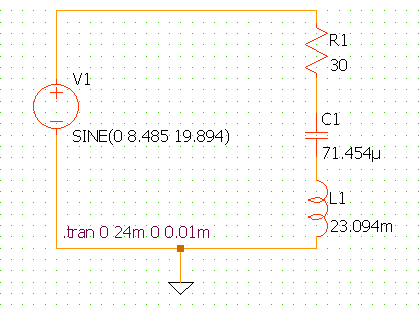
\includegraphics[width=1\textwidth]{./data/schema6}
	\caption{Схема замещения Двухполюсника 6 в LTspice.}
\end{figure}
\subsubsection{Расчётные формулы и расчёты}
\begin{enumerate}
	\item Расчёт действующего тока в цепи:
	      \[
		      \begin{gathered}
			      I = \frac{U}{Z} = \frac{U}{\sqrt{R^2 + X^2}} \\
			      X = X_L-X_C, R = R_1 + R_k \implies I = \frac{U}{\sqrt{(R_1+R_k)^2+(X_L-X_C)^2}} = \\
			      = \frac{6}{\sqrt{(30+5)^2+(2.887-111.96)^2}} = 0.0524 \, \text{А}
		      \end{gathered}
	      \]
	\item Расчёт фазового сдвига:
	      \[
		      \phi = \arctan\left(\frac{X_L-X_C}{R_1+R_k}\right) = \arctan\left(\frac{2.887-111.96}{30+5}\right) = -72.209^{\circ}
	      \]
\end{enumerate}

\subsubsection{Вектора входного напряжения и тока}

\[
	\begin{gathered}
		I_x = I \cos(\phi), I_y = I sin(\phi) \\
		I_x = 0.0524 \cdot \cos(72.209^\circ) = 0.016 \, \text{А}, \quad
		I_y = 0.0524 \cdot \sin(72.209^\circ) = 0.05 \, \text{А}
	\end{gathered}
\]
\begin{figure}[H]
	\centering
	\begin{tikzpicture}[scale=27.0]

		% Draw the grid
		\draw[very thin, gray] (-0.04,-0.2) grid (0.63,0.3);

		% Draw the axes
		\draw[->] (-0.04,0) -- (0.61,0) node[right] {$+1$};
		\draw[->] (0,-0.2) -- (0,0.3) node[above] {$+j$};

		% Draw the current vector (red) with a phase shift of -75 degrees
		\draw[->, red, thick] (0,0) -- ({0.0524*cos(-72.209)}, {0.0524*sin(-72.209)})
		node[end, right] {$I = 0.0524 \, \text{А}$};
		\draw[gray, thin, dashed] ({0.0524*cos(-72.209)},0) node[start, above, red] {\scriptsize0.016} -- ({0.0524*cos(-72.209)}, {0.0524*sin(-72.209)});
		\draw[gray, thin, dashed] (0,{0.0524*sin(-72.209)}) node[start, left, red] {\scriptsize0.05} -- ({0.0524*cos(-72.209)}, {0.0524*sin(-72.209)});


		% Draw the voltage vector (blue) for voltage (U)
		\draw[->, blue, thick] (0,0) -- (0.58,0) node[end, above] {$U = 6 \, \text{В}$};

		% Draw the phase angle arc (from U to I)
		\draw[thick] (0.03,0) arc[start angle=0, end angle=-72.209, radius=0.03];
		\node at (0.065,-0.025) {\small $\phi = 72.209^\circ$};

		% Labels for the axis
		\node[below left] at (0.005,0.005) {\scriptsize$0$};

	\end{tikzpicture}
\end{figure}


\subsection{Двухполюсник 7}
\subsubsection{Схема исследуемой цепи}
\begin{figure}[H]
	\centering
	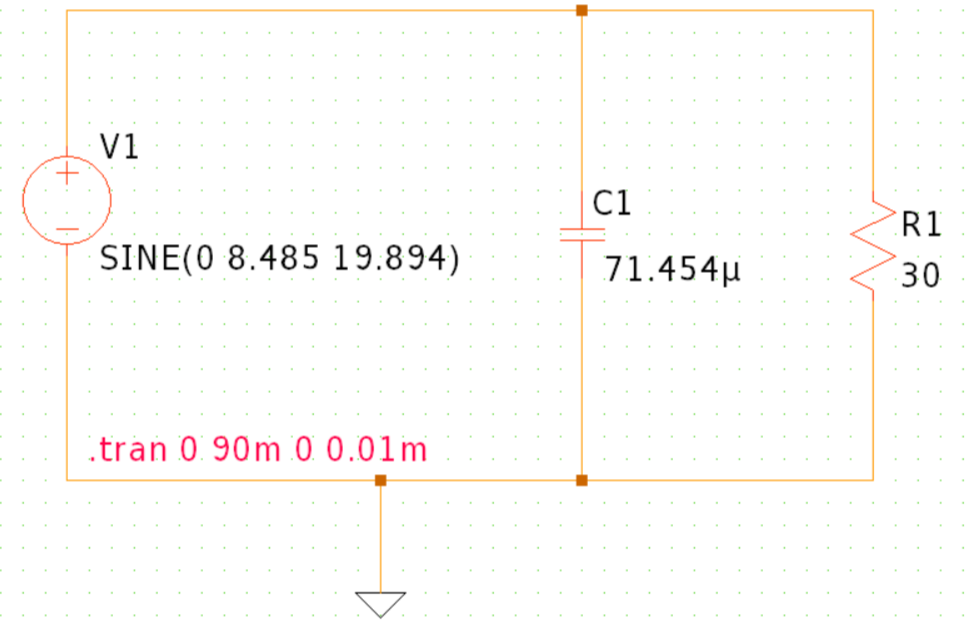
\includegraphics[width=1\textwidth]{./data/schema7}
	\caption{Схема замещения Двухполюсника 7 в LTspice.}
\end{figure}
\subsubsection{Расчётные формулы и расчёты}
\begin{enumerate}
	\item Расчёт действующего тока в цепи:
	      \[
		      \begin{gathered}
			      I = U \cdot Y = U \cdot \sqrt{G^2 + B^2} \\
			      G = \frac{1}{R_1}, B = -B_C \implies I = U \cdot \sqrt{\frac{1}{R_1^2} + B_C^2} = 6 \cdot \sqrt{\frac{1}{30^2} + 0.00893^2} = 0.207 \, \text{А}
		      \end{gathered}
	      \]
	\item Расчёт фазового сдвига:
	      \[
		      \phi = \arctan\left(\frac{-B_C}{\frac{1}{R_1}}\right) = \arctan\left(\frac{-0.00893}{0.03}\right) = -16.577^{\circ}
	      \]
\end{enumerate}

\subsubsection{Вектора входного напряжения и тока}
\[
	\begin{gathered}
		I_x = I \cos(\phi), I_y = I sin(\phi) \\
		I_x = 0.207 \cdot \cos(16.577^\circ) = 0.198 \, \text{А}, \quad
		I_y = 0.207 \cdot \sin(16.577^\circ) = 0.059 \, \text{А}
	\end{gathered}
\]
\begin{figure}[H]
	\centering
	\begin{tikzpicture}[scale=27.0]

		% Draw the grid
		\draw[very thin, gray] (-0.04,-0.2) grid (0.63,0.3);

		% Draw the axes
		\draw[->] (-0.04,0) -- (0.61,0) node[right] {$+1$};
		\draw[->] (0,-0.2) -- (0,0.3) node[above] {$+j$};

		% Draw the current vector (red) with a phase shift of -75 degrees
		\draw[->, red, thick] (0,0) -- ({0.207*cos(16.577)}, {0.207*sin(16.577)})
		node[end, right] {$I = 0.207 \, \text{А}$};
		\draw[gray, thin, dashed] ({0.207*cos(16.577)},0) node[start, above, red] {\scriptsize0.198} -- ({0.207*cos(16.577)}, {0.207*sin(16.577)});
		\draw[gray, thin, dashed] (0,{0.207*sin(16.577)}) node[start, left, red] {\scriptsize0.059} -- ({0.207*cos(16.577)}, {0.207*sin(16.577)});


		% Draw the voltage vector (blue) for voltage (U)
		\draw[->, blue, thick] (0,0) -- (0.58,0) node[end, above] {$U = 6 \, \text{В}$};

		% Draw the phase angle arc (from U to I)
		\draw[thick] (0.03,0) arc[start angle=0, end angle=16.577, radius=0.03];
		\node at (0.065,0.007) {\scriptsize $\phi = 16.577^\circ$};

		% Labels for the axis
		\node[below left] at (0.005,0.005) {\scriptsize$0$};

	\end{tikzpicture}
\end{figure}


\subsection{Двухполюсник 8}
\subsubsection{Схема исследуемой цепи}
\begin{figure}[H]
	\centering
	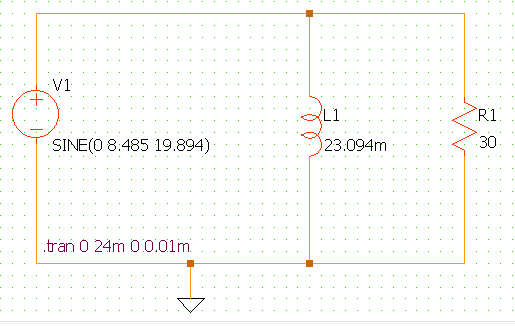
\includegraphics[width=0.7\textwidth]{./data/schema8}
	\caption{Схема замещения Двухполюсника 8 в LTspice.}
\end{figure}
\subsubsection{Расчётные формулы и расчёты}
\begin{enumerate}
	\item Расчёт действующего тока в цепи:
	      \[
		      \begin{gathered}
			      I = U \cdot Y = U \cdot \sqrt{G^2 + B^2} \\
			      G = G_1+G_k, B = B_k-B_1 \implies I = U \cdot \sqrt{(G_1+G_k)^2+(B_k-B_1)^2} = \\
			      = U \cdot \sqrt{\left(\frac{1}{R_1}+\frac{R_k}{R_k^2+X_L^2}\right)^2+\left(\frac{X_L}{R_k^2+X_L^2}-0\right)^2} = \\
			      = 6 \cdot \sqrt{\left(\frac{1}{30}+\frac{5}{5^2+2.887^2}\right)^2+\left(\frac{2.887}{5^2+2.887^2}\right)^2} = 1.217 \, \text{А}
		      \end{gathered}
	      \]
	\item Расчёт фазового сдвига:
	      \[
		      \phi = \arctan\left(\frac{B_k-B_1}{G_1+G_k}\right) = \arctan\left(\frac{0.0866}{0.183}\right) = 25.325^{\circ}
	      \]
\end{enumerate}

\subsubsection{Вектора входного напряжения и тока}
\[
	\begin{gathered}
		I_x = I \cos(\phi), I_y = I sin(\phi) \\
		I_x = 1.217 \cdot \cos(-25.325^\circ) = 1.1 \, \text{А}, \quad
		I_y = 1.217 \cdot \sin(-25.325^\circ) = -0.521 \, \text{А}
	\end{gathered}
\]
\begin{figure}[H]
	\centering
	\begin{tikzpicture}[scale=3.5]

		% Draw the grid
		\draw[very thin, gray] (-1.2,-1.2) grid (2.2,2.2);

		% Draw the axes
		\draw[->] (-1.2,0) -- (2.2,0) node[right] {$+1$};
		\draw[->] (0,-1.2) -- (0,2.2) node[above] {$+j$};

		% Draw the current vector (red) with a phase shift of -75 degrees
		\draw[->, red, thick] (0,0) -- ({1.217*cos(-25.325)}, {1.217*sin(-25.325)})
		node[end, right] {$I = 1.217 \, \text{А}$};
		\draw[gray, thin, dashed] ({1.217*cos(-25.325)},0) node[start, above, red] {\small1.1} -- ({1.217*cos(-25.325)}, {1.217*sin(-25.325)});
		\draw[gray, thin, dashed] (0,{1.217*sin(-25.325)}) node[start, left, red] {\small-0.521} -- ({1.217*cos(-25.325)}, {1.217*sin(-25.325)});


		% Draw the voltage vector (blue) for voltage (U)
		\draw[->, blue, thick] (0,0) -- (0.6,0) node[end, above] {$U = 6 \, \text{В}$};

		% Draw the phase angle arc (from U to I)
		\draw[thick] (0.18,0) arc[start angle=0, end angle=-25.325, radius=0.18];
		\node at (0.5,-0.07) {\scriptsize $\phi = 25.325^\circ$};

		% Labels for the axis
		\node[below left] at (0,0) {$0$};

	\end{tikzpicture}
\end{figure}


\subsection{Двухполюсник 9}
\subsubsection{Схема исследуемой цепи}
\begin{figure}[H]
	\centering
	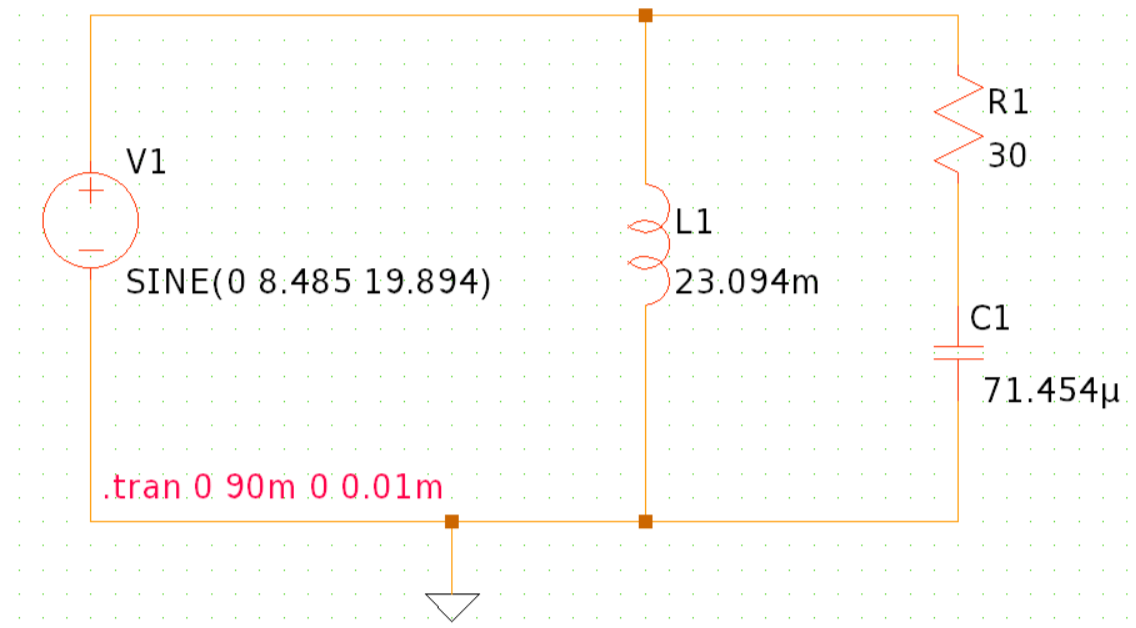
\includegraphics[width=1\textwidth]{./data/schema9}
	\caption{Схема замещения Двухполюсника 9 в LTspice.}
\end{figure}
\subsubsection{Расчётные формулы и расчёты}
\begin{enumerate}
	\item Расчёт действующего тока в цепи:
	      \[
		      \begin{gathered}
			      I = U \cdot Y = U \cdot \sqrt{G^2 + B^2} \\
			      G = G_1+G_k, B = B_k-B_1 \implies I = U \cdot \sqrt{(G_1+G_k)^2+(B_k-B_1)^2} = \\
			      = U \cdot \sqrt{\left(\frac{R_1}{R_1^2+X_C^2}+\frac{R_k}{R_k^2+X_L^2}\right)^2+\left(\frac{X_L}{R_k^2+X_L^2}-\frac{X_C}{R_1^2+X_C^2}\right)^2} = \\
			      = 6 \cdot \sqrt{\left(\frac{30}{30^2+111.96^2}+\frac{5}{5^2+2.887^2}\right)^2+\left(\frac{2.887}{5^2+2.887^2}-\frac{111.96}{30^2+111.96^2}\right)^2} = \\
			      = 1.027 \, \text{А}
		      \end{gathered}
	      \]
	\item Расчёт фазового сдвига:
	      \[
		      \phi = \arctan\left(\frac{B_k-B_1}{G_1+G_k}\right) = \arctan\left(\frac{0.0783}{0.152}\right) = 27.254^{\circ}
	      \]
\end{enumerate}

\subsubsection{Вектора входного напряжения и тока}
\[
	\begin{gathered}
		I_x = I \cos(\phi), I_y = I sin(\phi) \\
		I_x = 1.027 \cdot \cos(-27.254^\circ) = 0.913 \, \text{А}, \quad
		I_y = 1.027 \cdot \sin(-27.254^\circ) = -0.47 \, \text{А}
	\end{gathered}
\]
\begin{figure}[H]
	\centering
	\begin{tikzpicture}[scale=3.5]

		% Draw the grid
		\draw[very thin, gray] (-1.2,-1.2) grid (2.2,2.2);

		% Draw the axes
		\draw[->] (-1.2,0) -- (2.2,0) node[right] {$+1$};
		\draw[->] (0,-1.2) -- (0,2.2) node[above] {$+j$};

		% Draw the current vector (red) with a phase shift of -75 degrees
		\draw[->, red, thick] (0,0) -- ({1.027*cos(-27.254)}, {1.027*sin(-27.254)})
		node[end, right] {$I = 1.027 \, \text{А}$};
		\draw[gray, thin, dashed] ({1.027*cos(-27.254)},0) node[start, below, red] {\small0.913} -- ({1.027*cos(-27.254)}, {1.027*sin(-27.254)});
		\draw[gray, thin, dashed] (0,{1.027*sin(-27.254)}) node[start, left, red] {\small-0.47} -- ({1.027*cos(-27.254)}, {1.027*sin(-27.254)});


		% Draw the voltage vector (blue) for voltage (U)
		\draw[->, blue, thick] (0,0) -- (0.6,0) node[end, above] {$U = 6 \, \text{В}$};

		% Draw the phase angle arc (from U to I)
		\draw[thick] (0.18,0) arc[start angle=0, end angle=-27.254, radius=0.18];
		\node at (0.5,-0.07) {\scriptsize $\phi = 27.254^\circ$};

		% Labels for the axis
		\node[below left] at (0,0) {$0$};

	\end{tikzpicture}
\end{figure}


\subsection{Заполненная таблица 2.2}

\subsection{Выводы}
